\section{Lösungsansatz zur Klassifikation}
In diesem Kapitel geht es um den gewählten Ansatz, wie eine Klassifikation der
Hunderassen für den großen (120 Klassen) und den kleinen (5 Klassen) Datensatz
mittels mehrerer Neuronaler Netze und eines Random Forest erreicht werden kann.

\subsection{Größe der Bilder}
\label{sec:größe-bilder}

% \begin{figure}
%   \centering
%   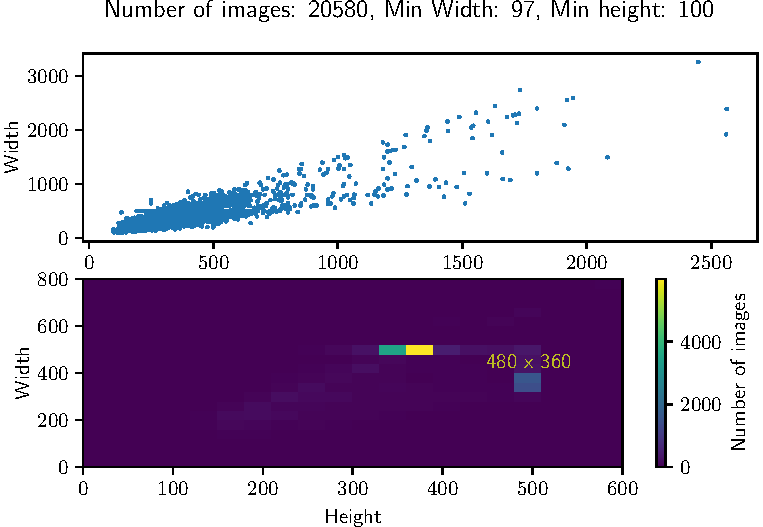
\includegraphics[scale=0.9]{pics/width_height_scatter_hist2d.pdf}
%   \caption{Oben: Scatter-Plot der Höhen- und Breitenverteilung der Bilder aus dem großen Datensatz.
%   Unten: Zweidimensionales Histogramm der Höhen- und Breitenverteilung.
%   Die gelbe Größe entspricht der am häufigsten auftretenden Kombination
%   aus Breite und Höhe.}
%   \label{fig:scatter_groß}
% \end{figure}

Höhe und Breite der Bilder sind unterschiedlich im großen Datensatz, wie in
\autoref{fig:scatter_groß} dargestellt. Die minimale Breite liegt bei 97 Pixeln
und die minimale Höhe bei 100 Pixeln bzw. für den kleinen Datensatz bei 125x138
Pixeln. Prinzipiell arbeiten die verwendeten Neuronalen Netze ohne definierte
Input size, allerdings müssen die Bilder aufgrund der Verwendung von
\texttt{numpy arrays} auf eine definierte Größe gebracht werden. Eine
Möglichkeit wäre es nun, alle Bilder auf diese minimale Größe zu reskalieren. Damit
würde allerdings ein Informationsverlust einhergehen. Aus diesem Grund wurde für
\MiniDog{} (mehr dazu in \autoref{sec:netzwerk}) ein zu Teilen
selbstgeschriebener \texttt{Datagenerator} verwendet, der die Bilder batchweise
lädt und batchweise auf das Minimum im Batch reskaliert. Auf diese Weise ist der
Informationsverlust geringer als alle Bilder auf 125x138 zu reskalieren.

% \begin{figure}
%   \centering
%   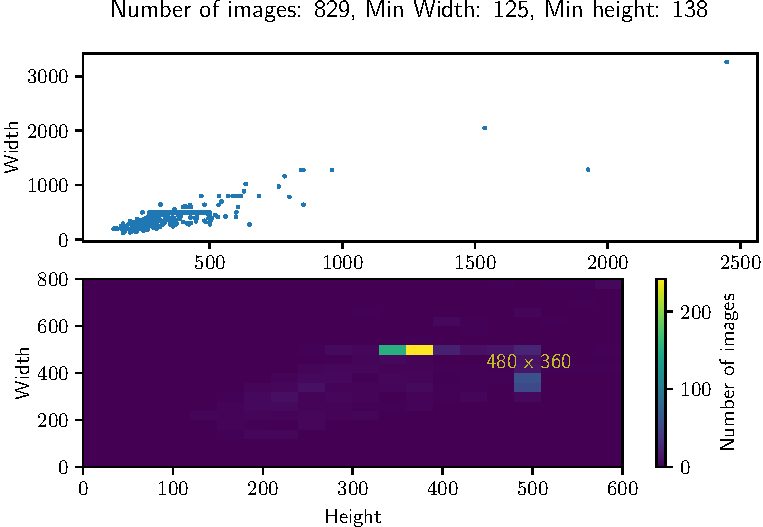
\includegraphics[scale=0.9]{pics/width_height_scatter_hist2d_klein.pdf}
%   \caption{Oben: Scatter-Plot der Höhen- und Breitenverteilung der Bilder aus
%   dem kleinen Datensatz.
%   Unten: Zweidimensionales Histogramm der Höhen- und Breitenverteilung.
%   Die gelbe Größe entspricht der am häufigsten auftretenden Kombination
%   aus Breite und Höhe.}
%   \label{fig:scatter_klein}
% \end{figure}

In \autoref{fig:scatter_klein} ist die Höhen- und Breitenverteilung auch für
den kleinen Datensatz dargestellt.
Für \PreDog{} und \PreBig{} (mehr in \autoref{sec:netzwerk}) muss aufgrund der
vortrainierten Netze eine feste Größe (224x224) der Bilder gewählt werden.
% Wegen technischen Schwierigkeiten konnte nicht auf die minimale Größe des großen
% Datensatzes trainiert  werden. Stattdessen wurde auf die minimale Größe des
% kleinen Datensatzes resized. Da nur maximal 71 Bilder des großen Datensatzes
% eine kleinere Größe haben als 125x138, fällt dies nicht allzu sehr ins Gewicht.

\subsection{Data Augmentation}
Wie bereits in \autoref{chap:datensatz} dargestellt, entfallen auf jede Klasse
nur ungefähr 150 Bilder, was eine sehr geringe Statistik darstellt. Aus diesem
Grund wurde Data Augmentation verwendet. Das bedeutet, dass bei jedem neuen
Aufruf des \texttt{Datagenerators} nach dem Reskalieren das Bild um einen zufälligen
Winkel zwischen \SI{-30}{\degree} und \SI{30}{\degree} rotiert wird. Dabei
aufstehende Leerflächen werden geschwärzt. Dann wird mit \SI{50}{\percent}
Wahrscheinlichkeit das Bild in x- und y-Richtung verschoben oder ein Zoom in x-
und y-Richtung durchgeführt. Damit bei diesen Transformationen der Hund noch
immer komplett zu sehen ist und nicht z.\,B. durch die Verschiebung nur noch ein
Teil des Hundes zu sehen ist, wird vorher aufgrund der Bounding Boxes, die im
Datensatz gegeben sind, das Zoom- bzw. Translationslimit bestimmt.

\begin{figure}
  \centering
  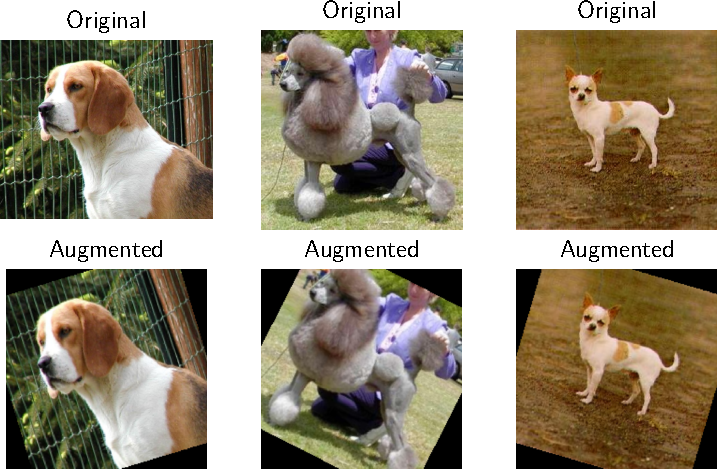
\includegraphics[scale=0.8]{pics/subplot.pdf}
  \caption{Beispielbilder zur Data Augmentation. In der oberen Zeile sind die
  Originalbilder aus dem Datensatz und unten die Bilder nach dem Reskalieren und der Data Augmentation.}
  \label{fig:data_augmentation}
\end{figure}

Drei Beispiele sind in \autoref{fig:data_augmentation} zu sehen.
Da der Datagenerator nach jeder Epoche neu aufgerufen wird, sehen die
Trainingsbilder in jeder Epoche anders aus, was allgemein die Robustheit der
Architekturen gegenüber Translation, Rotation, etc. erhöht und mehr
Statistik generiert, da die Bilder immer anders aussehen.

\subsection{Netzwerkstrukturen}
\label{sec:netzwerk}
Insgesamt wurden drei verschiedene Netzwerkarchitekturen verwendet, namentlich
\MiniDog{}, \PreDog{} (für den großen Datensatz) und \PreBig{} (für den kleinen
Datensatz). Die letzten beiden Architekturen verwenden dabei den
\texttt{Convolutional Neural Network (CNN)}-Anteil eines vortrainiertes Netzes
mit Namen \texttt{InceptionResNetV2}. Dieses ist bei Keras vorimplementiert
\cite{inception} und wurde auf \texttt{ImageNet} trainiert, einem Datensatz
insgesamt bestehend aus 14197122 Bildern \cite{imagenet}. Auf das vortrainierte
\CNN{} folgt ein zu trainierendes \texttt{Fully Connected Network (FNC)}.
Aus dem \CNN{} werden 1536 Features generiert, die bei der Verwendung von Farbinformationen
zu 47255 zu trainierenden Gewichten für \PreDog{} und zu 249545 zu trainierenden Gewichten
für \PreBig{} führen. Diese große Anzahl bedingt, dass Regularisierung verwendet werden
muss; in diesem Fall \texttt{L2-Regularisierung} und \texttt{Dropout}.

Die Struktur ist für beide Neuronalen Netze die gleiche: An
\texttt{InceptionResNetV2} ist eine Lage \texttt{AveragePooling2D} mit einer
\texttt{Poolsize=(4, 4)} und eine Lage \texttt{GlobalMaxPooling\-2D}
angeschlossen, um die Anzahl der freien Parametern für den \FNC{}-Layer
festzulegen. Danach kommen drei \texttt{Dense}-Layer, mit den Dimensionalitäten
30, 30, 5 (für \PreDog{}) und 150, 120, 120 (für \PreBig{}). Die Layern sind
\texttt{L2-Regularisiert} mit einem Wert von 0.007 für beide Architekturen.
Außerdem befinden sich je ein \texttt{Dropout}-Layer mit einer Stärke von 0.15
zwischen den \texttt{Dense}-Layern. Die Aktivierungsfunktion der
\texttt{Dense}-Layer ist \texttt{PReLU}, die Initialisierung wurde nach der von
Kaiming He entwickelten Methode durchgeführt \cite{tensowflow-he}, so wie in
\cite{he-ini} empfohlen. Auch die Gewichte des Kernels der \texttt{Dense}-Layer
wurden nach der von Kaiming He entwickelten Methode initialisiert.
\texttt{PReLU} ist eine modifizierte Version von \texttt{ReLU}, die sich dadurch
auszeichnet, dass die Funktion $f(y)$ für negative $y$ nicht 0 ist wie bei
\texttt{ReLU}, sondern $ay$ mit einem Koeffizienten $a$, der adaptiv angepasst
wird \cite{prelu}. Die Aktivierungsfunktion des letzten \texttt{Dense}-Layers
ist \texttt{softmax}, da diese Funktion normiert ist und das Ergebnis somit als
Wahrscheinlichkeit der Klassenzugehörigkeit interpretiert werden kann
\cite[S. 139]{hands_on_machine_learning}.

\begin{figure}
  \centering
  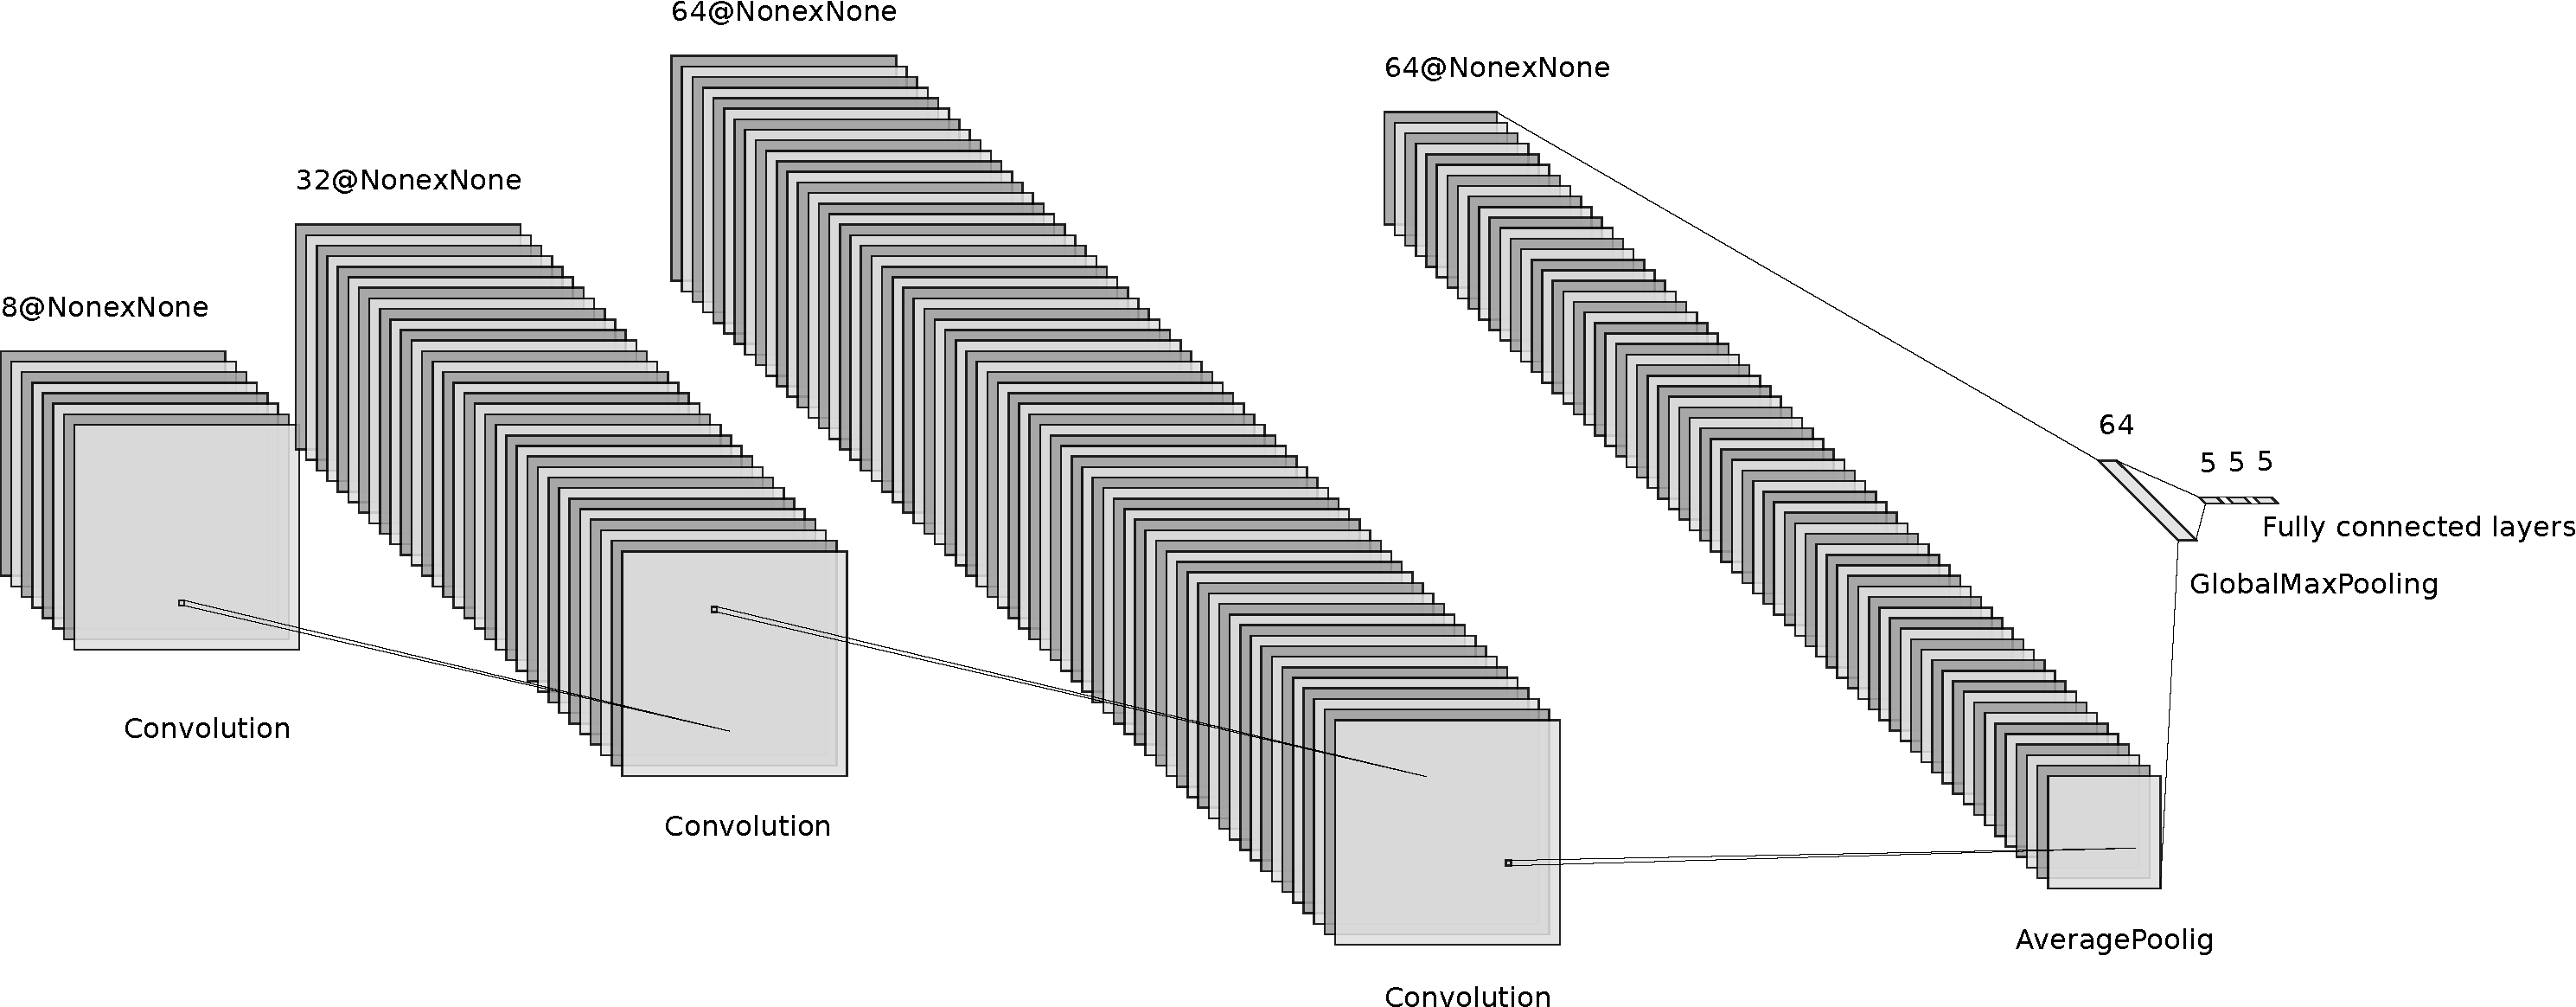
\includegraphics[width=\textwidth]{pics/nn.pdf}
  \caption{Struktur des Neuronalen Netzes \MiniDog{}. Die Dimensionalität
  der \texttt{Dense}-Layer richtet sich nach der Anzahl der Klassen im verwendeten Datensatz.}
  \label{fig:struktur_minidognn}
\end{figure}

Außerdem wurde ein Neuronales Netz ohne vortrainiertes Netz verwendet, dies heißt
\MiniDog{}. Die Struktur ist in \autoref{fig:struktur_minidognn} abgebildet.
Wie schon bei \PreDog{} und \PreBig{} wird für die \texttt{Dense}-Layer und auch
für die \texttt{Convolutional}-Layer wird die von Kaiming He entwickelte Methode
zur Initialisierung der Gewichte verwendet. Ebenso wird \texttt{PReLU} als
Aktivierungsfunktion genutzt für beide Arten von Layern. Außerdem wird
\texttt{L2-Regularisierung} für alle Arten von Layern genutzt.

Als letzte Netzwerkstruktur wird der Autoencoder und der dazugehörige Random
Forest vorgestellt. Der Encoder des Autoencoders besteht aus vier
\texttt{Convolutional}-Layern mit drei \texttt{MaxPooling}-Layern dazwischen,
die die Auflösung der Bilder reduzieren. Mit dem \texttt{flatten}-Layer wird
dafür gesorgt, dass die Bilder am Ende des Encoders statt als dreidimensionales
Array als Vektor vorliegen. Der Decoder besteht aus fünf
\texttt{Convolutional}-Layern und drei \texttt{UpSampling2D}-Layern, die
zwischen den ersten vier \texttt{Convolutional}-Layern platziert sind und die
Auflösung der Bilder wieder steigern; also die inverse Transformation zu den
\texttt{MaxPooling}-Layern durchführen. Zu Beginn des Decoders wird mit einem
\texttt{Reshape}-Layer aus dem Vektor wieder ein dreidimensionales Array
gemacht. Die Aktivierungsfunktionen der \texttt{Convolutional}-Layer ist
\texttt{ReLU}, bis auf den letzten, dort wird \texttt{Sigmoid} verwendet, da
alle Pixelwerte auf eins normiert sind und der Wertebereich der Funktion
zwischen null und eins liegt.

\subsection{Hyperparameter-Optimierung}
\label{sec:hyperparam}
Für \MiniDog{} und der Random Forest wurde eine Hyperparameter-Optimierung in Form
eines \texttt{Grid Search} durchgeführt.
Dabei wurden die Stärke der \texttt{L2-Re\-gu\-la\-ri\-sier\-ung} $\in \{0.01,
0.001, 0.005, 0.0001\}$, die \texttt{Batch-Size} $\in \{2, 5, 10, 15, 17, 25\}$
und das Verwenden der Farbinformationen $\in \{True, Fal\-se\}$ als Parameter
verwendet und in den angegebenen Räumen variiert. Von diesem 48 möglichen
Kombinationen konnten nur 43 erfolgreich trainiert werden, da die restlichen
aufgrund von Grafikspeicherproblemen beendet wurden. Die \texttt{Epochenanzahl}
und die \texttt{learning rate} wurden nicht variiert, da \texttt{EarlyStopping}
bzw. \texttt{ReduceLROnPlateau} verwendet wurden; also beide Parameter im
Verlaufe des Trainings dynamisch angepasst wurden.
Für den \RF{} wurden \texttt{GridSearchCV} mit einer dreifachen Kreuzvalidierung
genutzt, siehe \autoref{tab:hyper_rf}. Unter anderem wurde die maximale Tiefe oder die Anzahl an Schätzern
optimiert. Für eine Hyperparameter-Optimierung von \PreBig{} und \PreDog{} in
der gegebenen Zeit war die Hardware nicht stark genug.
% Allerdings wurde im Falle von \MiniDog{}
% eine selbgeschriebene Funktion verwendet, die aus Zeitgründen auf die
% \texttt{Cross Validation} verzichtet. Auch werden nur drei Hyperparameter
% optimiert: Die Stärke der \texttt{L2-Re\-gu\-la\-ri\-sier\-ung}, die
% \texttt{Batch-Size} und das Verwenden der Farbinformationen. Beim letzten Punkt
% werden die Bilder einmal in schwarz-weiß und einmal mit Farbinformationen
% eingelesen, um zu prüfen, wie wichtig dieser Parameter für das Neuronale Netz
% ist.

% \begin{table}
%   \caption{Optimierte Hyperparameter für den \RF}
%   \label{tab:hyper_rf}
%   \begin{tabular}{c c c c c c}
%     \toprule
%     max\_features & max\_depth & min\_samples\_leaf & min\_samples\_split & criterion & n\_estimators \\
%     \midrule
%     auto, log2 & None, 10, 100 & 1, 10 31 & 2, 8, 10 & gini, entropy & 100, 400, 1000, 1500 \\
%     \bottomrule
%   \end{tabular}
% \end{table}
